% Supplement fragment. Compile from the supplement/ directory.
\section{S-Core: Platform, Metric, and Relationship Evidence Profiles}
\label{supp:core}

\subsection{Platform Assignment}

The main-text platform table retains the canonical mutually exclusive family
counts for 206 studies. Each study is assigned to its dominant physical
platform, while physical media and integration mechanisms can overlap within
the same system. Transmitters supplied through fiber enter the photonic
terahertz family when photonic generation and conversion create the wireless
carrier directed at the target. Fiber remains the organizing platform when it
transports signals to downstream RFID, radio, or radar sensing. Hybrid
membership requires interaction across segments to shape the result. Family
counts describe corpus coverage rather than relative performance or maturity.

\subsection{Metric Evidence}

The primary synthesis contains 4,779 metric records. A record is an extraction
unit preserving a reported quantity, its available definition, conditions, and
source location; it is not an independent study or effect estimate. Data rate,
BER, and range resolution appear in 85, 60, and 50 studies, respectively, with
overlapping study coverage.

\begin{table}[htbp]
\caption{Domain coverage of the primary metric records}
\label{tab:s_metric_domains}
\centering
\footnotesize
\setlength{\tabcolsep}{4pt}
\begin{tabular}{@{}lrr@{}}
\toprule
Domain & Records, $n$ (\%) & Studies, $n$ (\%) \\
\midrule
Sensing & 1,816 (38.0\%) & 203 (98.5\%) \\
Communication & 1,328 (27.8\%) & 194 (94.2\%) \\
Joint & 870 (18.2\%) & 158 (76.7\%) \\
Implementation & 476 (10.0\%) & 64 (31.1\%) \\
Smaller normalized domains & 289 (6.0\%) & 33 (16.0\%) \\
\bottomrule
\end{tabular}
\end{table}

Domain rows partition the primary metric records, whereas study counts overlap.
Of these records, 118 (2.5\%) are conditional comparison candidates and 4,661
(97.5\%) retain their native-context analytical role. Candidate status requires
the reported definition, task, measurement plane, operating conditions, and
validation to be checked before any proposed comparison. It does not establish
a verified comparison across independent studies or justify pooling. The
remaining records support mechanism, feasibility, and qualitative synthesis in
their source contexts. The complete metric register contains 4,861 rows,
including 31 contextual records and 51 records documenting source conflicts.
Electronic Supplement S-Evidence preserves the complete records and provenance.

\subsection{Joint Performance Relationships}

The relationship register contains 404 entries. Two document the absence of a
tradeoff, leaving 402 substantive relationships from 168 studies. These include
218 quantitative and 184 qualitative records; 371 substantive relationships
have condition-dependent interpretations. The profile in
Fig.~\ref{fig:s_tradeoff_profile} preserves the overlapping mechanism-family
coverage. A relationship is not a study, a pooled effect, or an independently
verified cross-study comparison. The main text uses selected within-study
examples to explain how a shared choice changes communication and sensing.

\begin{figure*}[t]
\centering
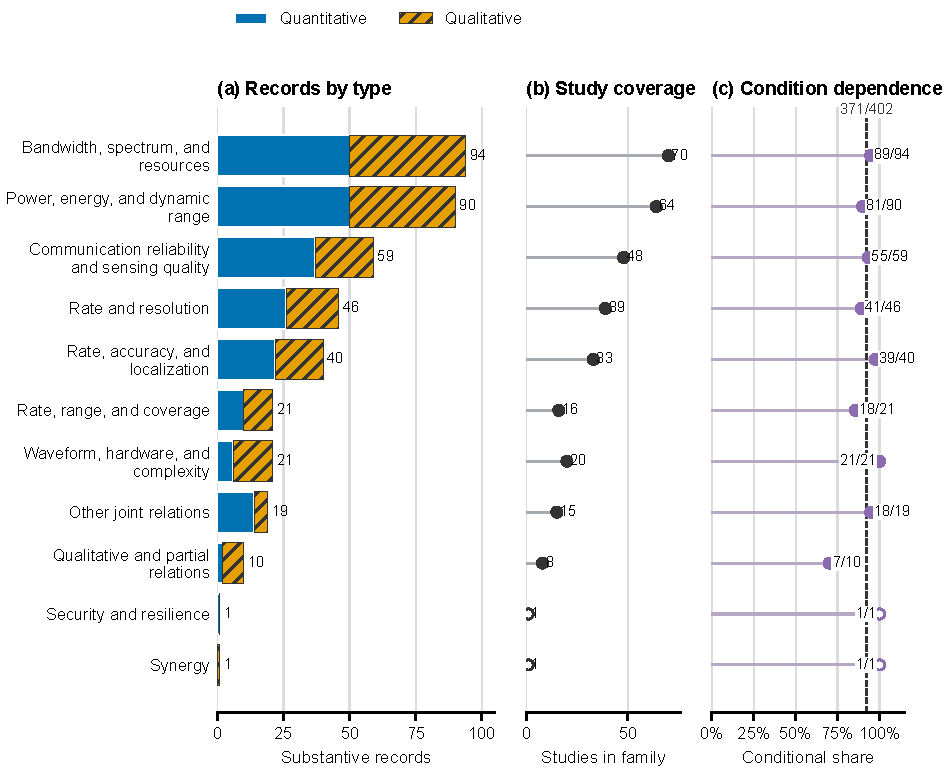
\includegraphics[width=\textwidth]{../manuscript/figures/final_submission_2026-08-25/fig06_tradeoff_profile.pdf}
\caption{Descriptive profile of the 402 substantive joint-performance
relationships. Panel (a) separates quantitative and qualitative records;
panel (b) reports overlapping study coverage across mechanism families;
panel (c) reports condition dependence. Family frequency describes corpus
coverage, not effect size or comparative maturity.}
\label{fig:s_tradeoff_profile}
\end{figure*}
